%%% Intro.tex --- 
%% 
%% Filename: Intro.tex
%% Description: 
%% Author: Ola Leifler
%% Maintainer: 
%% Created: Thu Oct 14 12:54:47 2010 (CEST)
%% Version: $Id$
%% Version: 
%% Last-Updated: Thu May 19 14:12:31 2016 (+0200)
%%           By: Ola Leifler
%%     Update #: 5
%% URL: 
%% Keywords: 
%% Compatibility: 
%% 
%%%%%%%%%%%%%%%%%%%%%%%%%%%%%%%%%%%%%%%%%%%%%%%%%%%%%%%%%%%%%%%%%%%%%%
%% 
%%% Commentary: 
%% 
%% 
%% 
%%%%%%%%%%%%%%%%%%%%%%%%%%%%%%%%%%%%%%%%%%%%%%%%%%%%%%%%%%%%%%%%%%%%%%
%% 
%%% Change log:
%% Completed Language Reading MBS
%% 
%% RCS $Log$
%%%%%%%%%%%%%%%%%%%%%%%%%%%%%%%%%%%%%%%%%%%%%%%%%%%%%%%%%%%%%%%%%%%%%%
%% 
%%% Code:


\chapter{Integration of Optimization tool-chain into the Model-Based Development Process}
\label{cha:optimization}

This chapter is based on the following paper:

\begin{itemize}
	
	\item \textbf{Alachew Shitahun}, Vitalij Ruge, Mahder Gebremedhin, Bernhard Bachmann, Lars Eriksson, Joel Andersson, Moritz Diehl, and Peter Fritzson. \textbf{Model-Based Optimization with OpenModelica and CasADi.} In Proceedings of IFAC Conference in Tokyo, September 2013. 
	
	\item  \textbf{Alachew Shitahun}, Vitalij Ruge, Mahder Gebremedhin, Bernhard Bachmann, Lars Eriksson, Joel Andersson, Moritz Diehl, Peter Fritzson. \textbf{Tool Demonstration Abstract: OpenModelica and CasADi for Model-Based Dynamic Optimization.} In Proceedings of the 5th International Workshop on Equation-Based Object-Oriented Modeling Languages and Tools, Nottingham, UK, April 19, 2013. 
		
\end{itemize}



\section{Introduction}
\label{sec:optimizationintroduction}

During the last decade, nonlinear model predictive control (NMPC) and non-linear optimal control problems (NOCP)
based on Differential-Algebraic Equations (DAEs) have had a significant impact in the industrial community, particularly in
the control engineering area \cite{biegler, tamimi}. State-of-the-art methods use numerical
algorithms for dynamic optimization based on direct multiple shooting \cite{bock} or collocation algorithms
\cite{biegler}.

Use of equation-based, object-oriented modeling languages such as Modelica for
industrial applications has increased. These languages enable users to conveniently model large-scale physical systems described by 
differential, algebraic, and discrete equations, primarily with the goal of performing virtual experiments (simulation) 
on these systems, but recently also optimization.

Due to the influence of such equation-based, object-oriented modeling languages in the industrial community, there have
been several attempts to integrate tools for such languages with numerical algorithms for optimization. For example,
Dymola \cite{dymola} supports parameter and design optimization of models written in Modelica, whereas
JModelica.org \cite{akesson} and OpenModelica \cite{bernhard} have native support for optimal
control.

This chapter presents results of an effort in which OpenModelica and CasADi \cite{casadi} have been integrated to perform model-based dynamic optimization. The problem formulation and modeling is done in Modelica 
including the optimization \cite{optimica} language extension. The integration is based
on standardized XML format presented in \cite{xml} for exchange of \acrshort{daes} models. 
OpenModelica supports export of models written in Modelica and the optimization language extension using this XML 
format, while CasADi supports importing of models represented in this format. This allows users to define optimal control problems (OCP) using
Modelica and optimization language specification, and solve the underlying model formulation using a
range of optimization methods, including direct collocation and direct multiple shooting. The proposed
solution has been tested on several industrially relevant optimal control problems, including a diesel-electric
power train.

\section{CasADi}
\label{sec:optcasadi}

CasADi \cite{casadi} is an open-source framework for C++ and Python that provides numerical optimization in general and optimal control in particular. The main idea of the tool is to provide users with the ability to easily and efficiently implement optimal control algorithms with a wide range of methods, including multiple shooting and collocation, rather than providing users with a “black-box” OCP solver.
The tool supports symbolic import of OCPs via an extended version of the functional mockup interface (FMI) format as explained in \cite{optandersson}. This OCP can then be transcribed into a nonlinear programming problem (NLP) and solved with one of CasADi’s interfaced NLP solvers.

\section{Modelica and the Optimization Language Extension}
\label{sec:optimizationoptimica}

Modelica is a mature and powerful language with regard to modeling of complex hybrid dynamical systems. However, it
lacks important features for describing or modeling optimization problems. This is not a surprise since Modelica
was not originally designed to help with dynamic optimization problems.

The optimization language extension \cite{optimica} complements Modelica by providing features that enable
formulation of dynamic optimization problems based on Modelica models. The optimization extension to Modelica
consists of the following elements:

\begin{itemize}
	
\item \textit{objective} and \textit{objectiveIntegerand}, which maps the Mayer and the Lagrange term in 
            the objective function respectively.
\item \textit{startTime}, which defines the start of the optimization interval.
\item \textit{finalTime}, which defines the end of the optimization interval.
\item A new section: \textit{constraint}, which defines inequality constraints.
\end{itemize}

The requirement and motivation for introducing these specific features is covered in more detail in \cite{optimica}.

\section{Modeling NOCP and XML Export in OpenModelica Compiler}
\label{sec:optimizationopenmodelica}

The OpenModelica compiler front-end has been extended to support the optimization language extension described in
Section \ref{sec:optimizationoptimica}. 

\begin{figure} [!h]
	\includegraphics[width=\linewidth]{opt_modeling_NOCP.png}
	\caption{Modeling NOCP using the OpenModelica Graphical and Textual Editor.}
	\label{fig:nocpmodel}
\end{figure}

This enables users to use the OpenModelica graphical editor (OMEdit) (see Figure \ref{fig:nocpmodel})to formulate and use model-based NOCP that can be solved by CasADi.
In addition, the OpenModelica compiler has recently been extended with XML export of models \cite{alachew} based on the XML
format defined in \cite{xml}. This schema is an extended version of the XML schema
defined by the Functional Mock-up Interface (FMI) \cite{fmi}, and is the most recent in a series of
Modelica-related XML schemas starting with ModelicaXML \cite{pop}. The XML export also includes the
optimization language extension, and OpenModelica is integrated with CasADi for the type of model-based dynamic optimization reported in this thesis.

\section{Complete Model-Based Dynamic Optimization tool-chain}
\label{sec:optimizationtoolchain}

Before exporting a Modelica and optimization language model to XML, the model should be symbolically
instantiated by the compiler in order to get a single flat system of equations. The model variables should also be
scalarized. The compiler front end performs this, including syntax checking, semantics and type checking, simplification
and constant evaluation, etc. Then the complete flattened model is exported to XML code. The exported
XML document can then be imported to CasADi for model-based dynamic optimization. The complete tool chain is
visualized in Figure \ref{fig:optimizationtoolchain}.


\begin{figure} [!h]
	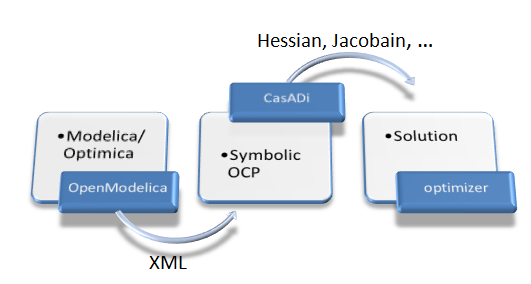
\includegraphics[width=\linewidth]{opt_tool_chain.png}
	\caption{Model-Based Dynamic Optimization tool-chain for OpenModelica and CasADi.}
	\label{fig:optimizationtoolchain}
\end{figure}

The XML will be imported and symbolically pre-processed in CasADi. In particular, the fully-implicit \acrshort{dae} from
Modelica is reformulated in a semi-explicit form. With the NOCP now available in CasADi’s native data structures, the
NOCP can be reformulated to a NLP as outlined in \cite{alachewoptimization} (See Section 2.2).

At the time of our work, the efficient symbolic pre-processing model evaluation from OpenModelica is not yet completely
implemented to import into CasADi. So the symbolic preprocessing in CasADi can be used. The symbolic work in CasADi makes it easy to create the goal function and constraints.

The NLP is solved by one of the NLP solvers interfaced to CasADi, e.g., IPOPT \cite{wachter}. First and second order derivative information will be generated by CasADi using automatic differentiation and passed to the solver.

\section{Testing the Tool-chain Implementation}
\label{sec:optimizationtesting}

In this section, we describe the solution of an industrially-relevant optimal control problem for a diesel-electric powertrain. The
formulation of the underlying optimization problem and the corresponding optimization results are presented in the
following subsections.

\subsection{Fuel optimal control of a diesel electric powertrain}
\label{sec:optimizationdiesel}

The diesel-electric powertrain model presented in \cite{sivertsson,bernhard} is a nonlinear
mean value engine model (MVEM) containing four states and three control inputs, while the generator model is
simplified by considering constant efficiency and maximum power over the entire speed range, see Figure \ref{fig:dieselmodel} for the
schematic diagram of the model.

\begin{figure} [!h]
	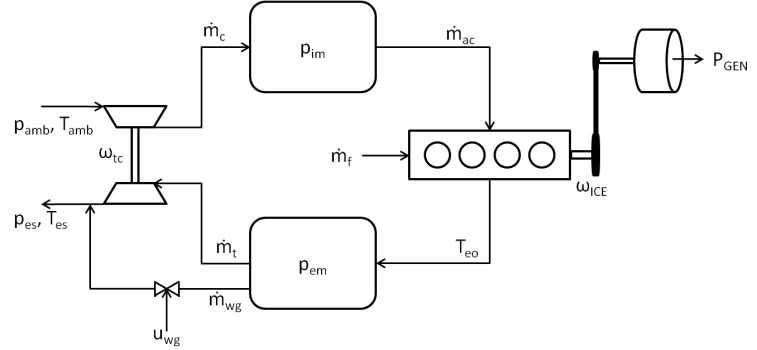
\includegraphics[width=\linewidth]{opt_diesel_model.png}
	\caption{Diagram of the diesel-electric powertrain model.}
	\label{fig:dieselmodel}
\end{figure}

In a diesel-electric powertrain the operating point of the diesel engine can be freely chosen, which would potentially
decrease fuel consumption. Moreover, the electric machine has better torque characteristics. These are the main reasons
that the diesel-electric power-train concept is interesting for further studies.

To investigate the fuel-optimal transients of the powertrain from idling condition to a certain power level while the
accelerator pedal position is interpreted as a power level request, the following optimal control problem is solved:

\begin{equation*}
 \begin{aligned}
	\text{states}\quad x = 0, \quad \begin{pmatrix} w_{ice} \\ p_{im} \\p_{em} \\w_{tc}  \end{pmatrix}\quad = \quad \text{controls,}\quad u = \begin{pmatrix} u_{f} \\ u_{wg} \\p_{gen} \\w_{tc}  \end{pmatrix} \\
	\text{min}\;\int_{0}^{T}\dot{m}{_f} d_t
\end{aligned}
\end{equation*}

subject to

\begin{equation*}
	\begin{aligned}
		\dot{x}_1 = f_2 (x_2,x_3,u_1,u_3 ) \\
		\dot{x}_2= f_3 (x_1,x_2,x_4 ) \\
		\dot{x}_3=f_4 (x_1,x_2,x_3,u_1,u_2 ) \\
		\dot{x}_4=f_5 (x_2,x_3,x_4,u_2 ) \\
		0= f_6 (x_2,x_4 )- f_7 (x_1,x_2 ) \\
		0= f_7(x_1,x_2 ) + f_8 (x_1,u_1 )-f_9 (x_3 )-f_{10}(x_3,u_3 )  \\
		0= \frac{f_{11}(x_3)-f_{12}(x_1 )} {f_{13}(x_4 )}-f_{14} (x_4 )
\end{aligned}
\end{equation*}

\begin{equation*}
	\begin{aligned}
      54 rps \;\leq  \;  x_1  \;\leq \; 220 rps \\
      0.8 p_{amp} \;\leq \;  x_2 \; \leq \; 2P_{amb} \\
      P_{amb} \;  \leq\; x_3 \;\leq \;  3P_{amb} \\
      300rps  \; \leq \; x_4 \;\leq \;   10000 rps \\
      0 \;\leq \;u_1,u_2 \;\leq \; 1
	\end{aligned}
\end{equation*}

and boundary conditions are:

\begin{equation*}
 \begin{aligned}
	\text{at}\quad t = 0,  \begin{pmatrix} x_1 \\ x_2 \\x_3 \\x_4  \end{pmatrix} = \text{idle operating values,} \\
	\text{at}\quad t = T,  \begin{pmatrix} \dot{x}_1 \\ \dot{x}_2 \\\dot{x}_3\\\dot{x}_4 \end{pmatrix} = 0,  \begin{pmatrix} x1 \\ x2 \\x3 \\x4  \end{pmatrix} = \text{desired values} \\
	\text{and}\quad v_3 = P_{required}.
 \end{aligned}
\end{equation*}

The constraints are originated from components’ limitations and the functions $ f_i$ are described in \cite{sivertsson}.

\subsection{Model import into CasADi and NLP transcription}
\label{sec:optimizationxmlimport}

We used OpenModelica to translate Modelica/ Optimization
language extension code into an OCP in DAE and Lagrange
cost function. This OCP is then exported into an XML-based
symbolic expression format and imported into CasADi via
OpenModelica. The OCP can then be transcribed into a
nonlinear programming problem (NLP) using the approach
outlined in \cite{bernhard} of Section 5, and solved with one of CasADi’s interfaced NLP solvers.

\subsection{Solution of the NLP}
\label{sec:optimizationnlp}

The NLP was solved using IPOPT \cite{wachter} running by default with the MUMPS linear solver.
The right scaling is important for a solution without oscillations.
On the other hand, if the scaling does not work in all steps
then changing of the solver tolerance is helpful. By itself, the diesel model
scales well in the time interval [0.32, 0.5],
which is the critical interval here.

In order to cover the optimal solution of the diesel-electric
powertrain model, 140 NLP iterations for 128 sub-intervals
with the total collocation (Lobatto6 and Radau5) are required by
IPOPT.

A better initial guess will change the NLP iterations.
Table \ref{tab:table1} shows the total CPU time for the optimization. The calculations have been done on a Dell Latitude E6410 laptop
with an Intel Core i7 processor of 2.8 GHz, 8 GB of RAM, 4M Cache, running Windows.

\begin{table} [!h]
\begin{center}
	\caption{Execution times for the diesel-electric powertrain model.} 
	\label{tab:table1} 
	\begin{tabular}{ cc } 
		\hline
		\bfseries Step & \bfseries Time  \\ 
		IPOPT (without function evaluation) & 2.140s \\ 
		NLP function evaluations & 1.158s \\ 
		\hline
	\end{tabular}
\end{center}
\end{table}

The control and state trajectories of the optimal solutions are shown in Figure \ref{fig:optimizationresultstatevariables} and Figure \ref{fig:optimizationresultcontrolvariables}, respectively. 

%%% \begin{figure} [!h]
%%%	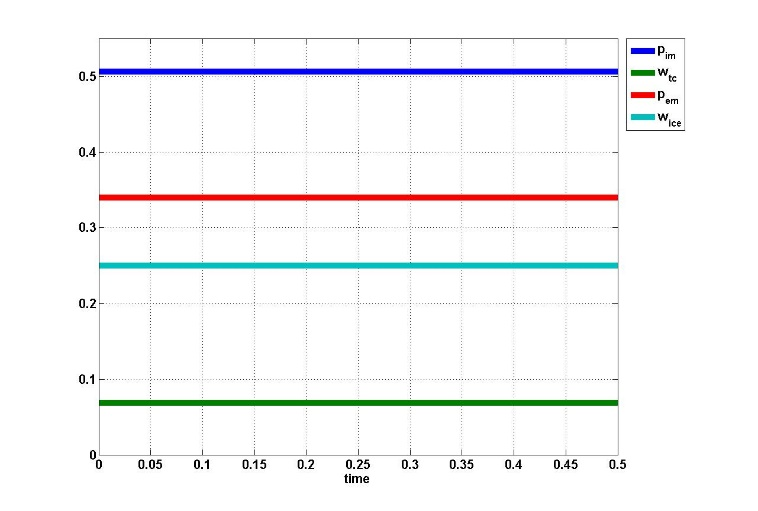
\includegraphics[width=\linewidth]{opt_initial_guess_state_variables.jpg}
%%%	\caption{Initial guess for diesel model - state variables.}
%%%	\label{fig:initialguessstatevariables}
%%% \end{figure}

%%% \begin{figure} [!h]
%%%	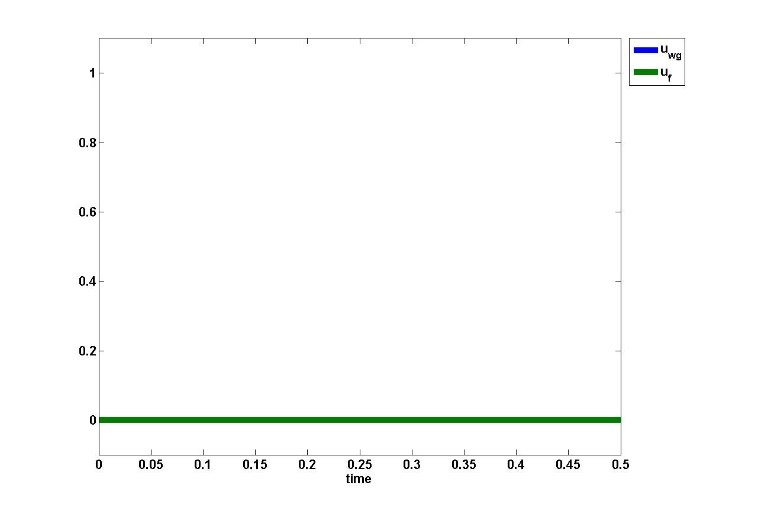
\includegraphics[width=\linewidth]{opt_initial_guess_control_variables.jpg}
%%%	\caption{Initial guess for diesel model - control variables.}
%%%	\label{fig:initialguesscontrolvariables}
%%% \end{figure}

The problem solved here is a minimum fuel problem for a transient from idle to 170 kW, for an end time of 0.5 s. For simplicity, only diesel operating condition is assumed which
means $(u_3=P_{gen} = 0)$. As expected, the fuel optimal results happen when the engine is accelerated only near the
end of the time interval $(t\approx 0.32 s)$, to meet the end constraints while minimizing the fuel consumption.

\begin{figure} [!h]
	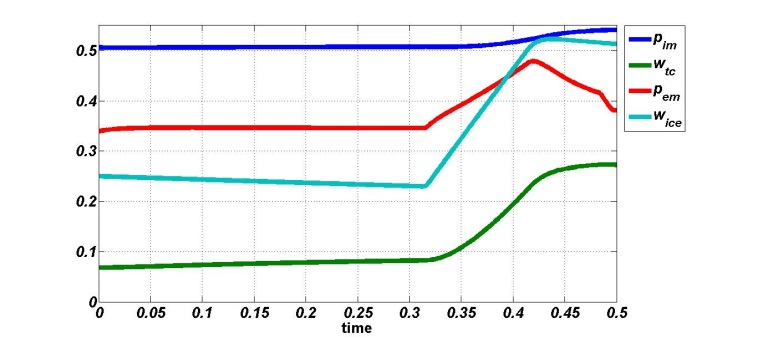
\includegraphics[width=\linewidth]{opt_result_state_variables.jpg}
	\caption{Optimization result for diesel model - state variables.}
	\label{fig:optimizationresultstatevariables}
\end{figure}

\begin{figure} [!h]
	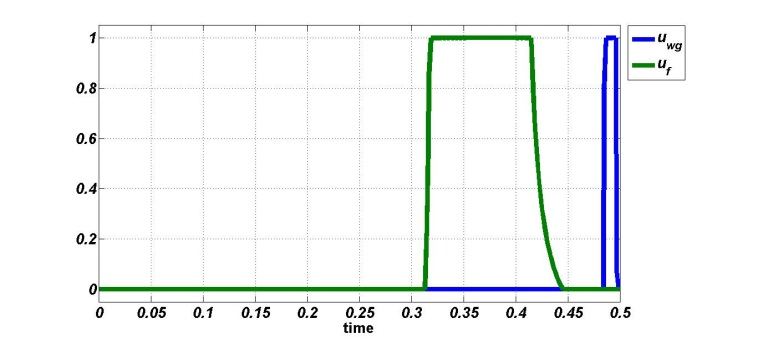
\includegraphics[width=\linewidth]{opt_result_control_variables.jpg}
	\caption{Optimization result for diesel model - control variables.}
	\label{fig:optimizationresultcontrolvariables}
\end{figure}

\clearpage
With amendments to the initial values, the process is robust. For this purpose, the initial values are changed slightly.

\begin{figure} [!h]
	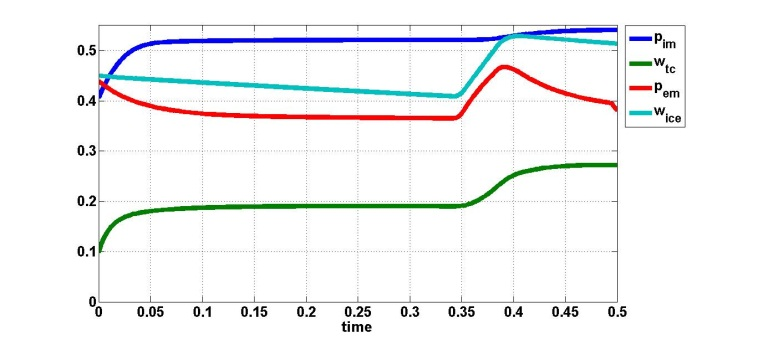
\includegraphics[width=\linewidth]{opt_result_state_variables_changed.jpg}
	\caption{Optimization result for diesel model with changed initial values - state variables.}
	\label{fig:optimizationresultchangedstatevariables}
\end{figure}

\begin{figure} [!h]
	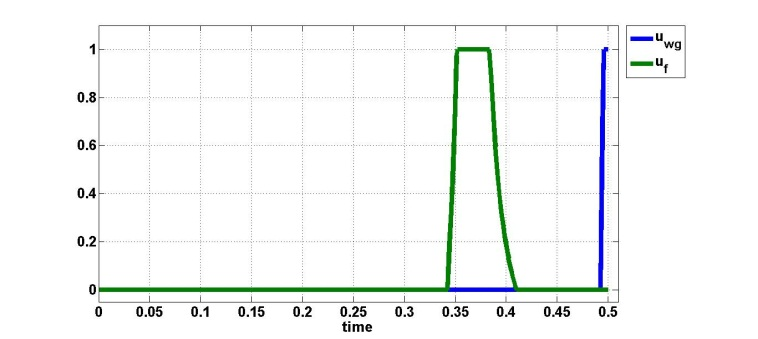
\includegraphics[width=\linewidth]{opt_result_control_variables_changed.jpg}
	\caption{Optimization result for diesel model with changed initial values - control variables.}
	\label{fig:optimizationresultchangedcontrolvariables}
\end{figure}

\clearpage
\section{Summary}
\label{sec:optimizationsummary}

This chapter demonstrates simulation-based optimization through the coupling of two open-source tools: OpenModelica, which is a Modelica-based modeling and simulation platform, and CasADi, a framework for numerical optimization. The coupling uses a standardized XML format for exchange of
differential-algebraic equations (DAE) models. OpenModelica supports export of models written in Modelica and the optimization language extension using this XML format, while CasADi supports import of models represented in this format. This allows users to define optimal control problems (OCP) using
Modelica and optimization language specification, and to solve the underlying model formulation using a range of optimization methods, including direct collocation and direct multiple shooting. The proposed solution has been tested on several industrially-relevant optimal control problems, including a diesel-electric power train.

\subsection*{Acknowledgements}
\label{sec:optimizationacknowledgements}

This work has been partially supported by Serc, by SSF in the EDOp project and by Vinnova as well as the German
Ministry BMBF (BMBF F\"{o}rderkennzeichen: 01IS09029C) in the ITEA2 OPENPROD project and in the ITEA2 MODRIO
project. The open-source Modelica Consortium supports the OpenModelica work.
JA and MD acknowledge support by PFV/10/002 OPTEC, GOA/10/09 and GOA/10/11, FWO G.0320.08, G.0377.09,
SBO LeCoPro; Belspo IUAP P7 DYSCO, FP7-EMBOCON (ICT-248940), SADCO (MC ITN-264735),
ERC ST HIGHWIND (259 166), Eurostars SMART, vicerp, ACCM.


%\nocite{scigen}
%We have included Paper \ref{art:scigen}

%%%%%%%%%%%%%%%%%%%%%%%%%%%%%%%%%%%%%%%%%%%%%%%%%%%%%%%%%%%%%%%%%%%%%%
%%% Intro.tex ends here


%%% Local Variables: 
%%% mode: latex
%%% TeX-master: "demothesis"
%%% End: 

